
%%%%%%%%%%%%%%%%%%%%%%%%%%%  5  %%%%%%%%%%%%%%%%%%%%%%%%%%% 
\section{A high-speed network interface for distributed-memory systems: architecture and applications \cite{steenkiste1997high}} \label{ss:steenkiste1997high}
%%%%%%%%%%%%%%%%%%%%%%%%%%%  5  %%%%%%%%%%%%%%%%%%%%%%%%%%% 

\Accs{dmm} have not been successful in using the \acc{hippi} protocol.
Applications on distributed systems tend to have very diverse I/O requirements.
% \Ac{hippi} support a data rate of 1.6 Gb/second. in traditional shard-memory supercomputers.
The problem lies in the high-speed I/O for \ac{dmm}, because the systems work optimally in a distributed fashion while connected to an inherent sequential (I/O) system.
An approach to network I/O on \ac{dmm} is to make the network interface (see: \cref{fig:rep4:conndistrmem}) responsible for network processing.
However, this is hard to do, because of potentially thousands of connected processor.
This approach could be improved by doing a selection of the communication overhead sensitive activities on the \ac{dmm}.

\begin{figure}[H]
    \centering
	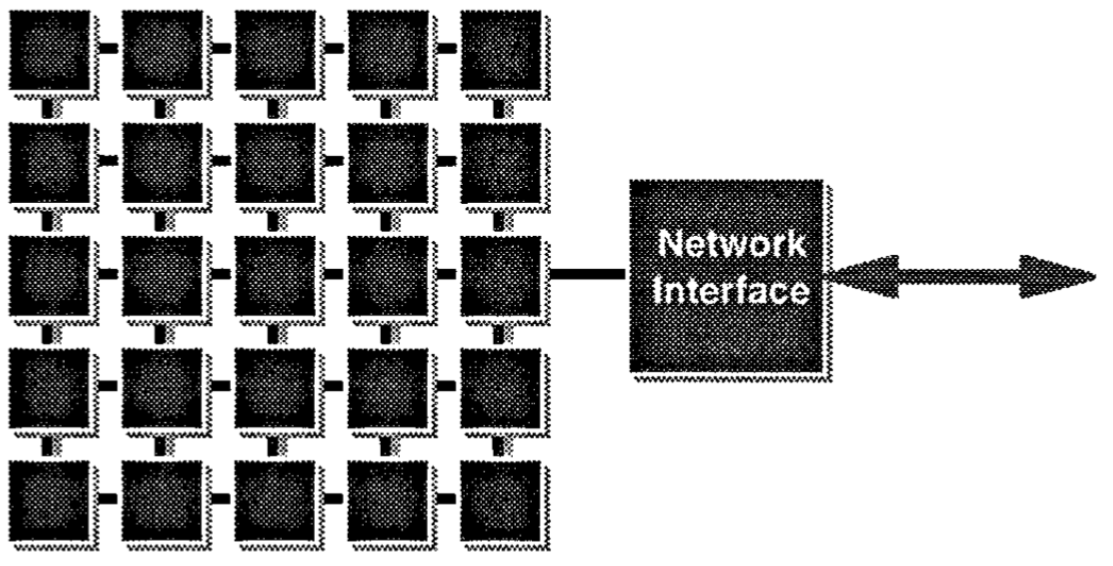
\includegraphics[width=0.95\linewidth]{Figures/Rep4DistrMemSys.png}
	\caption{Connecting a distributed-memory system to a network., Source: \cite{steenkiste1997high}.} 
    \label{fig:rep4:conndistrmem}
\end{figure}

% \motive
% There is a bottleneck in communication on \acs{dmm} which needs to be reduced.

\objective
An I/O architecture is created that supports high-speed I/O using a simple network interface to solve this problem.

\summary
\Ac{dmm}s communicate through a network interface that is connected both to the external network and the internal interconnect of the system (see: \cref{fig:rep4:conndistrmem}).



% High speed I/O for \ac{dmm} is difficult because the system is designed to operate in a distributed fashion where serialization is avoided as much as possible.
It is hard to implement the following tasks on a \ac{dmm}: the communication protocol (does not parallelize well), resource scheduling, data collection (data is typically divided between the private memories of the individual nodes). 
These tasks roughly correspond to the OSI network model (see: \cref{fig:rep4:osi}).
Additional problems are that some \acs{dmm} have slower internal links than the high-speed local-area networks such as \ac{hippi}.
Furthermore, applications on \ac{dmm} have diverse I/O requirements.

\begin{figure}
    \centering
	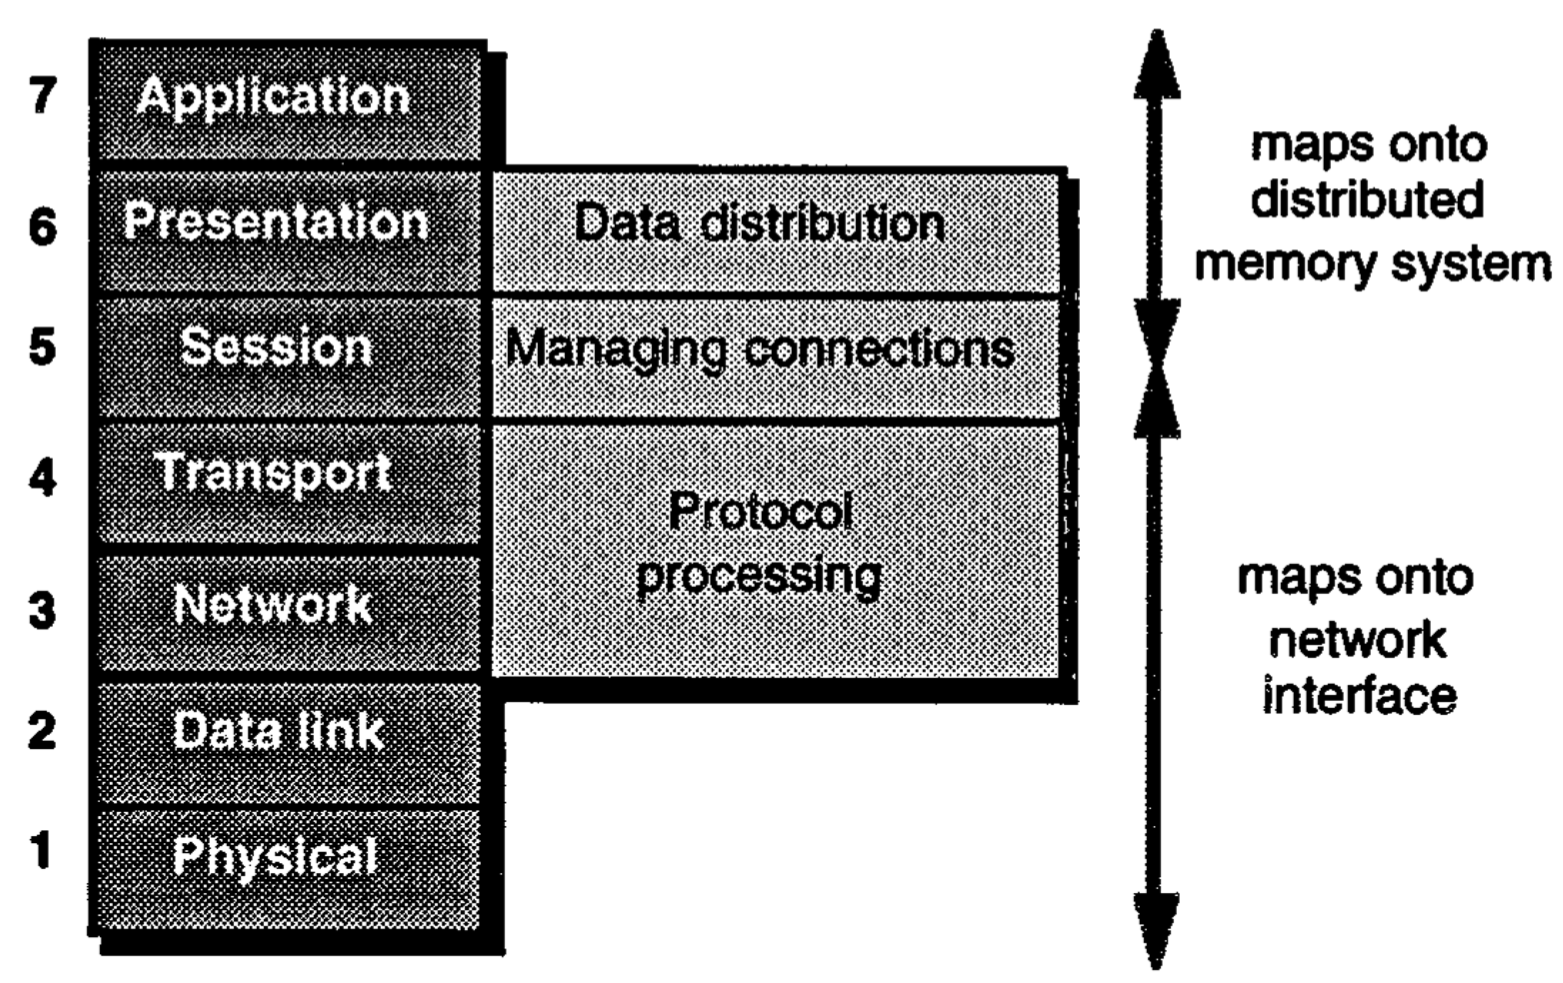
\includegraphics[width=0.95\linewidth]{Figures/Rep4OSI.png}
	\caption{Mapping of the protocol stack., Source: \cite{steenkiste1997high}.} 
    \label{fig:rep4:osi}
\end{figure}

%2.2 Architecture
\subsection{Architecture}
The designed I/O architecture allows the communication tasks to be performed on the \ac{dmm} as much as possible in combination with a network interface (\acc{hib}, see: \cref{fig:rep4:hib}).
The communication tasks are mapped in the following ways:
\begin{itemize}
    \item Processing of the transport and network protocol is performed on the (serial) network interface (\ac{hib}).
    \item The network interface provides an I/O interface that can be implemented efficiently on the network interface.
    \item The \ac{dmm} combines the distributed data on the private memories to large blocks for the network interface to process.
\end{itemize}

This mappings allows for appropriate scaling with network speed and data complexity.
This architecture is implemented for the iWarp system and a \ac{hippi} network.

%3 iWarp overview
\subsection{iWarp overview}
The iWarp system is a distributed-memory parallel computing system and combines high-speed computation and a communication agent in one component.
The communication agent connects an iWarp cell to four iWarp cell neighbours (see: \cref{fig:rep4:torus}).

\begin{figure}
    \centering
	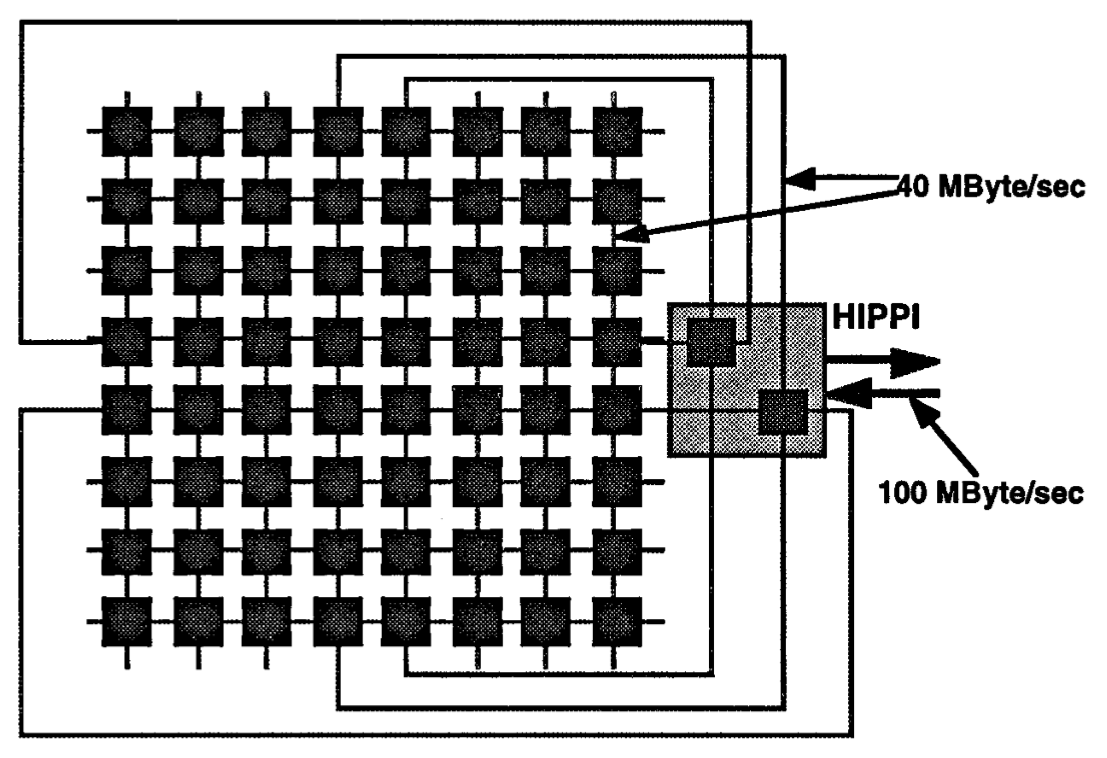
\includegraphics[width=0.95\linewidth]{Figures/Rep4torus.png}
	\caption{The \ac{hippi} network interface connected to the iWarp \ac{dmm}, also called the \textit{torus}., Source: \cite{steenkiste1997high}.} 
    \label{fig:rep4:torus}
\end{figure}

iWarp systems communicate with their external environment through I/O nodes linked to the torus (see: \cref{fig:rep4:torus}).
Applications produce output by sending data over the internal interconnect to the I/O node.

%4. Transport protocol processing
\subsection{Transport protocol processing}
Protocol processing is an potential bottleneck in network communication, it is inherently sequential.
There are two general categories in which protocol processing can be divided: overhead associated with every packed sent and overhead that scales with the number of bytes.
The later will dominate as networks get faster.
The solution lies in making these operations efficient by minimizing the number of times the data is touched.

%4.2 network interface architeutre
\begin{figure}
    \centering
	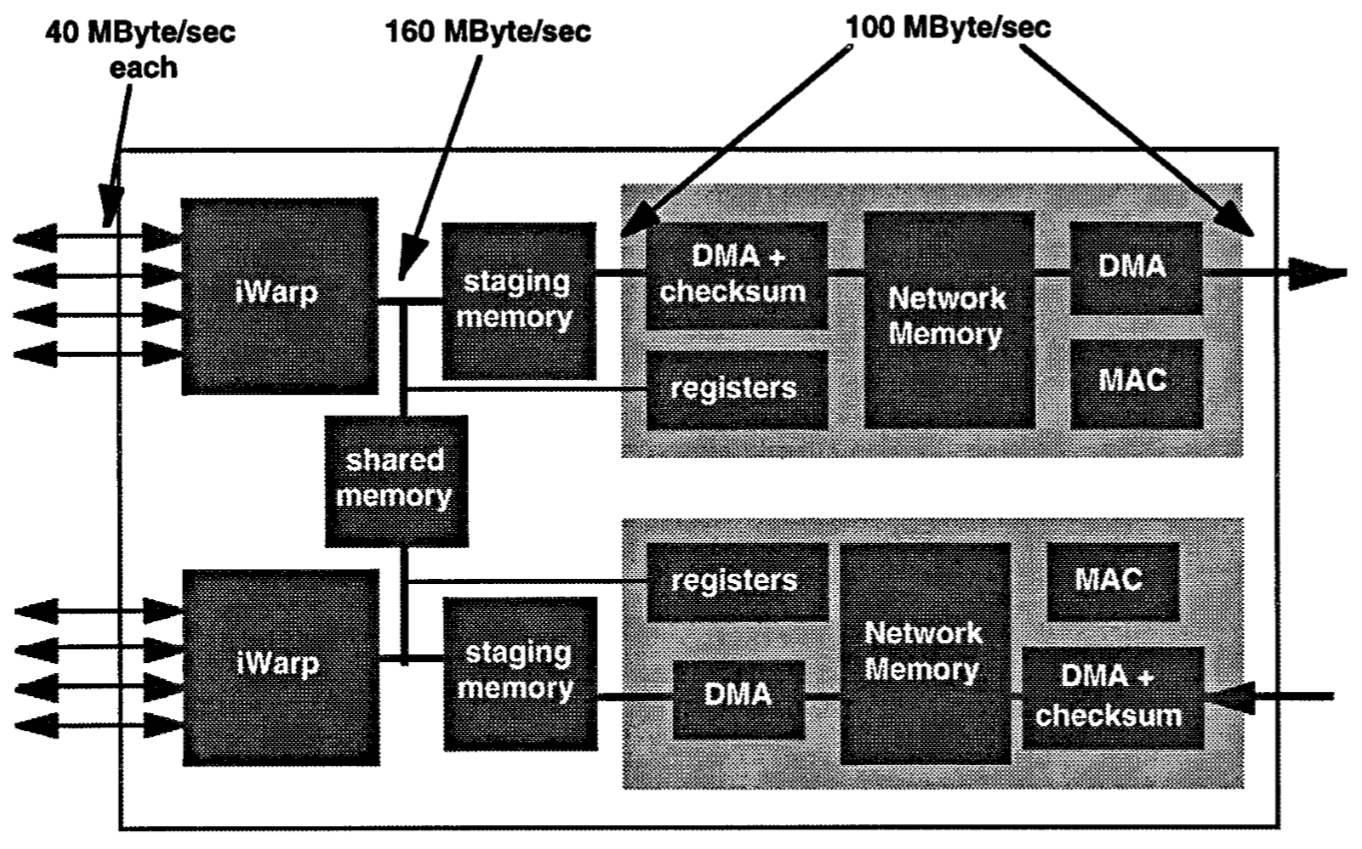
\includegraphics[width=0.95\linewidth]{Figures/Rep4hib.png}
	\caption{The \ac{hippi} interface Board Architecture. The gray areas show the communication acceleration blocks, Source: \cite{steenkiste1997high}.}
    \label{fig:rep4:hib}
\end{figure}

In \cref{fig:rep4:hib} the \ac{hib} is shown.
In the architecture the iWarp processor is responsible for per-packet operations, while the \acc{cab} (gray areas) is responsible for the per-byte operations.
%MS: missing connection with the CAB here
The high-bandwidth requirements typically make the memory bus the bottleneck of the network interface (\ac{hib}).
The \ac{hib} uses a couple of mechanisms to optimize the memory bandwidth utilization: it uses two iWarp processors (doubling of memory bandwidth) and the \ac{hib} uses two levels of memory optimized for different types of accesses.

% %Could have written something about 4.3 protocol software
% Measurement for raw \ac{hippi} and UDP over IP gave the same throughput results establishing that the UPD/IP implementation is very efficient.

% 5. THE STREAMS I/O ARCHITECTURE
\subsection{Streams I/O architecture}
There are two phases in which the transfer of data happens: the data is transferred from the distributed-memory system to the network interface and in the second phase data is transferred to the network.
Managing the first phase is a resource management problem which is tackled with the streams architecture (see: \cref{fig:rep4:streams}).

\begin{figure}
    \centering
	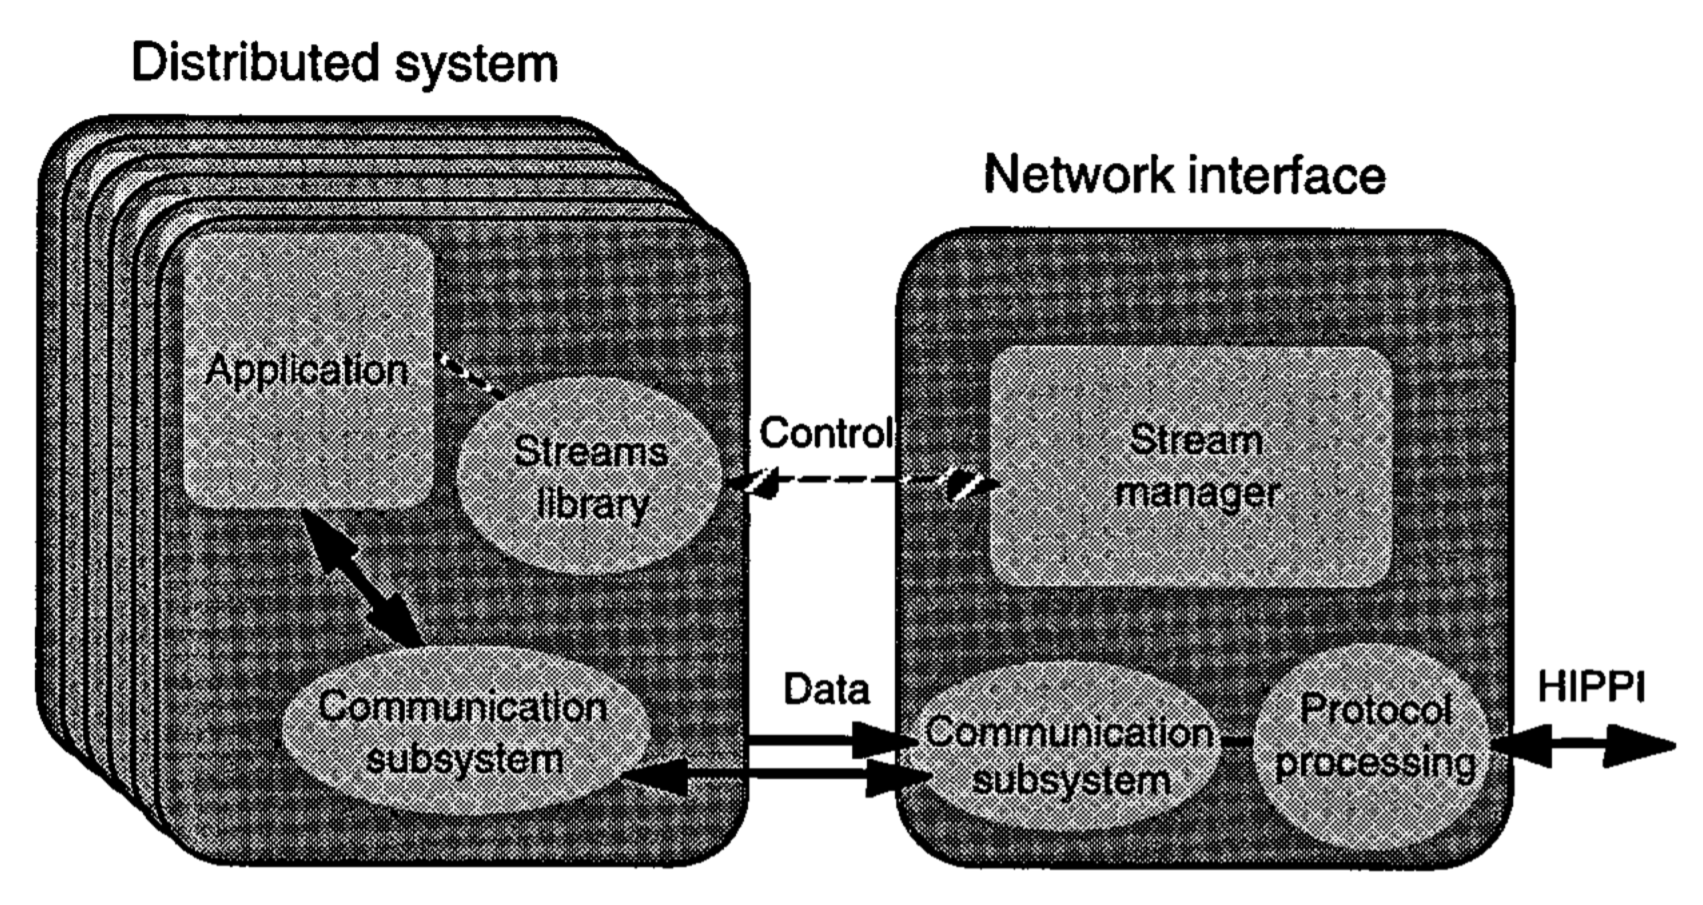
\includegraphics[width=0.95\linewidth]{Figures/Rep4streamsarchitecture.png}
	\caption{The stream architecture., Source: \cite{steenkiste1997high}.}
    \label{fig:rep4:streams}
\end{figure}

It is based on logical connections, each one supporting communication between the application on a \ac{dmm} to a destination on the external network.
A stream is defined as a data transfer on an established connection.
The application on the \ac{dmm} is responsible for distribution of the data to the network interface (\ac{hib}).
The \textit{stream manager} on the network interface is responsible for efficient data movement of multiple streams.

%5.2 dataformat
In the streams architecture the application provides the stream manager with information regarding the data format. 
This way the stream manager can plan and optimize the data transfers.

%5.3 iWarp streams software

%6. Data reshuffling in support of high-speed I/O
\subsection{Reshuffling}
Utilizing large number of processors requires data parallelism.
The data throughput depends on the number of links (due to striping) and the total message size.
Using data reshuffle, the throughput is optimized for different applications.

The \ac{dmm} is used for the scatter/gather operation.
This allows for the interface  node only to deal with large blocks of data and minimizes the cost on the network interface.

Also, reshuffling is an easy to parallelize operation which enables efficient reshuffle.
Parallelizing compilers have enough information to map a program onto a \ac{dmm} and provide it with the appropriate calls to do reshuffling.

%Conclusion
An architecture for network I/O is presented on \acs{dmm} and fast I/O rates over the iWarp \ac{hippi} interface were enabled.
This throughput was possible by a couple of key features: offloading of application specific tasks to the \ac{dmm}, the streams manager optimizes the network resource management.


